\chapter{Architecture}
 
\begin{figure}[!h]
\begin{center}
  \fbox{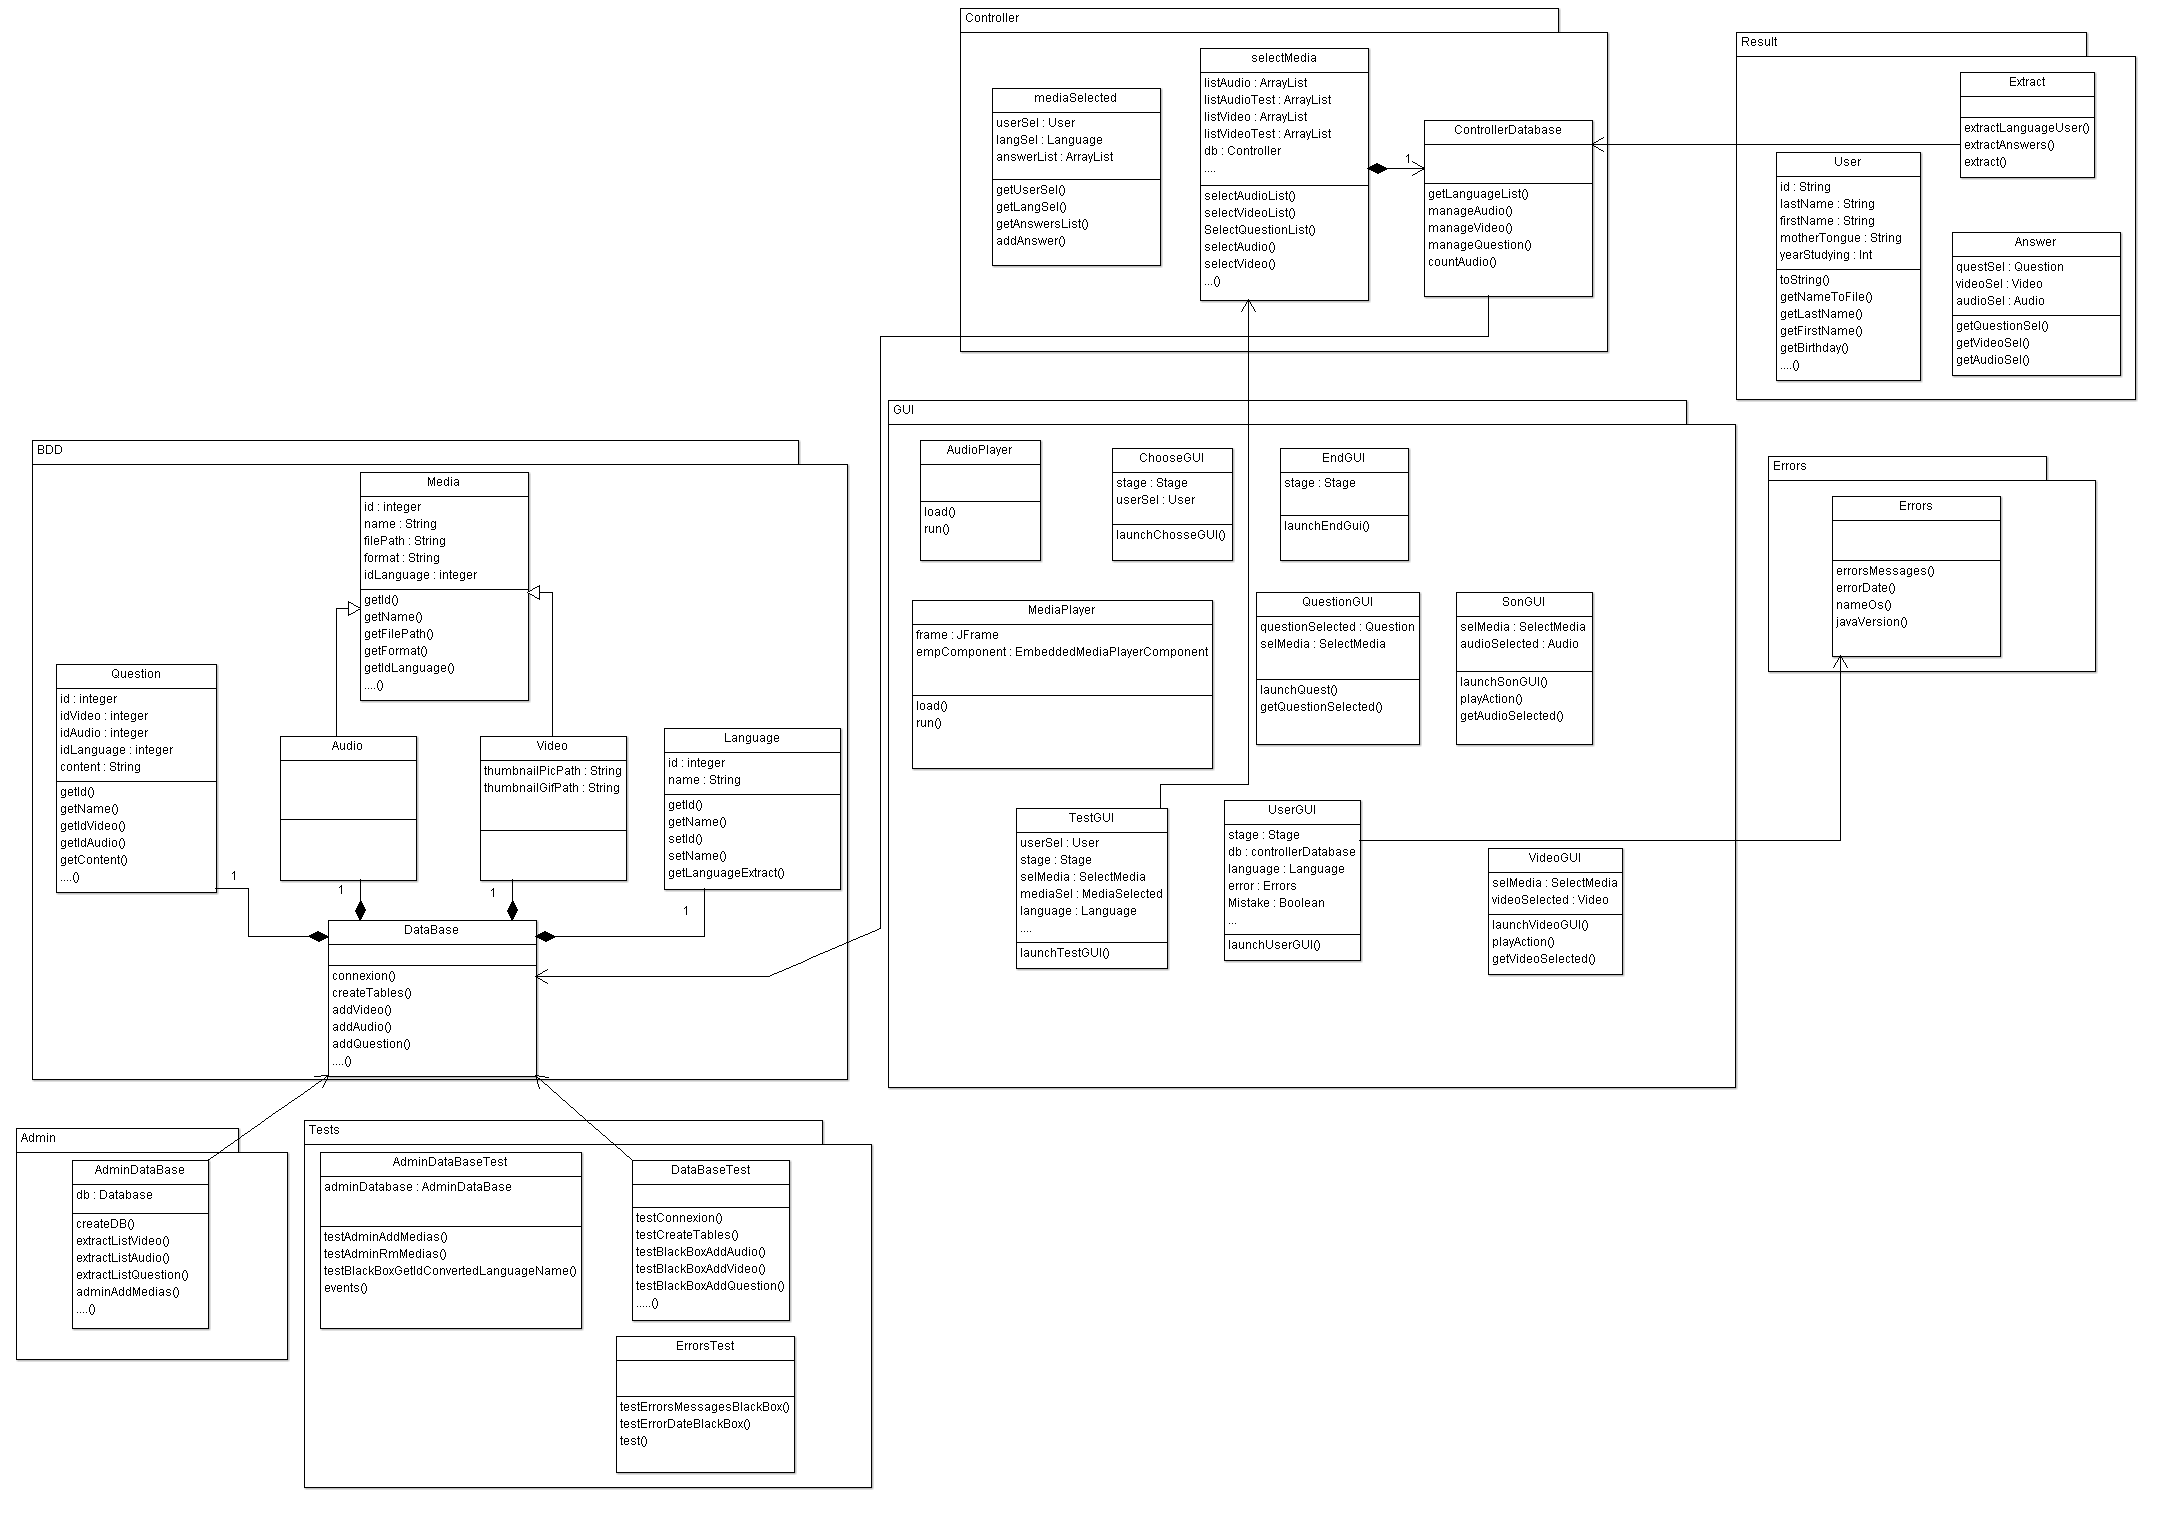
\includegraphics[width=18cm,angle=90]{./architecture/architecture.png}}
  \caption{UML - Architecture}
  \label{diaglog} 
\end{center}
\end{figure}

\section{Explication détaillée des packages}

Notre architecture est structuré en plusieurs packages. Ils ont été créés avec comme but de séparer notre architecture en fonction des besoins renseignés précédemment. Chaque package regroupe un certain nombre de classe possédant chacune une fonction bien précise. Dans cette section, nous allons décrire le besoin que nous avons voulu satisfaire avec le package et le rôle de chaque classe contenue dans le package.

\subsection{BDD}

On a créer ce package afin de regrouper les classes qui nous permette de gérer la base de données. En effet, notre base de données est consituée plusieurs entités comme les vidéos, les audios, les questions et enfin les langues. De ce fait, ce package contient l'ensemble des médias qui sera utilisé par l'application. Cette organisation des données a été choisie pour satisfaire et optimiser l'ajout de médias. De plus, si dans un futur proche, notre client souhaite intégrer une nouvelle langue pour ces tests, cet ajout sera simple et rapide.

\subsubsection{Classe DataBase}

Cette classe est très importante dans notre architecture. En effet, c'est elle qui est en lien direct avec la 

\subsubsection{Classes Media, Audio et Video}

\subsubsection{Classe Question}

\subsubsection{Classe Language}

\subsection{Result}

Ce package-ci est l'ensemble des informations concernant l'utilisateur (le sujet de l'expérience). Il est aussi composé de ses résultats aux réponses du test ainsi que d'une classe permettant d'extraire les données vers un fichier \textit{CSV / txt / XML}.

\subsection{Tests}

Ce package regroupe l'ensemble des tests qui seront necessaires pour minimiser les erreurs au niveau de la base de données (par exemple lors d'un upload de médias, on vérifie que le format soit adapté).

\subsection{Graphic}

Ici sont regroupés toutes les fonctionnalités liées à l'interface graphique.

\subsubsection{Classe UserGUI}

\subsubsection{Classe TestGUI}

\subsubsection{Classe ChooseGUI}

\subsubsection{Classe MediaManager}

\subsection{Processes}

Nous avons réuni ici, tout ce qui correspond au \textit{contrôleur} de l'application.

La classe \textbf{GUI\_select} est la sélection de l'ensemble des médias présentées lors d'une question.
\textbf{GUI\_Answer} correspond à la vidéo et à l'audio sélectionnés par l'utilisateur liés à une question.

\textbf{Cmd} est l'utilisation de l'application par l'administrateur lorsqu'il voudra ajouter ou retirer des médias et questions de la base de données.